\documentclass[10pt]{article}
\usepackage{mathpaper}
% \setpreview
\begin{document}
\showsecret
\papertitle{九年级上册期末质量检测一}
\paperinformation
\begin{questions}{\selectingintroduction}
    \question ``数学王子''高斯在19岁时发现了正十七边形的尺规作法,无论对他本人还是对数学界都是莫大的贡献,因此,人们在他的墓碑上刻上了正十七边形,作为永久的纪念.正十七边形(~~~~~~~).
    \twp{既是轴对称图形,又是中心对称图形}{是轴对称图形,但不是中心对称图形}{既不是轴对称图形,也不是中心对称图形}{是中心对称图形,但不是轴对称图形}
    \question 一元二次方程$2x^2+x-4=0$的两根之和为(~~~~~~~).
    \onp{$\frac{1}{4}$}{$-1$}{$-4$}{$-\frac{1}{2}$}
    \question 如图,四边形$ABCD$和$AEFG$均是正方形,连$BE$、$DG$,则下列说法中,不一定正确的是(~~~~~~~).
    \onp{$BE=DG$}{$BE \bot DG$}{$\angle EBC+\angle GDC=180^{\circ}$}{$\angle FEB=\angle GDC$}
    \question 掷两个质地均匀的骰子,则下列事件中,是随机事件的是(~~~~~~~).
    \twp{两骰子掷得的点数之和小于$13$}{两骰子掷得的点数之和等于$1$}{两骰子掷得的点数之差等于$4$}{两骰子掷得的点数之差等于$6$}
    \question 将抛物线$y=2x^2-8x+10$先向左平移$4$个单位长度,再向上平移$10$个单位长度得到的抛物线的解析式是(~~~~~~~).
    \twp{$y=2x^2-2x+16$}{$y=2x^2-24x+84$}{$y=2x^2+8x$}{$y=2x^2+8x+20$}
    \question 已知抛物线$y=ax^2-3ax-2a+1$与$y$轴交于负半轴,且过点$(1,y_1)$、$(3,y_2)$和$(-1,y_3)$,则$y_1$、$y_2$、$y_3$之间的大小关系是(~~~~~~~).
    \onp{$y_1<y_2<y_3$}{$y_3<y_2<y_1$}{$y_1<y_3<y_2$}{$y_3<y_1<y_2$}
    \question 用一根长$6$dm的细铁丝围一个矩形框架,则这个矩形的面积最大为(~~~~~~~)dm$^2$.
    \onp{$2$}{$2.25$}{$3$}{$9$}
    \question 如图,$AB$是$\odot O$的一条弦,过$B$作$\odot O$的切线$DB$(点$D$在点$B$的左侧),记$AB$的垂直平分线交优弧$\wideparen{AB}$于点$C$,连$AC$、$BC$,若$\angle DBA=40^{\circ}$,则$\angle CBA=$(~~~~~~~).
    \onp{$40^{\circ}$}{$80^{\circ}$}{$50^{\circ}$}{$70^{\circ}$}
    \question 如图,$PM$、$PN$分别切$\odot O$于$A$、$B$两点,$C$为$\odot O$上一点,连$AC$、$BC$.若$\angle P=60^{\circ}$、$\angle MAC=75^{\circ}$、$AC=\sqrt{3}+1$,则$\odot O$的半径长(~~~~~~~).
    \onp{$\sqrt{2}$}{$1$}{$\sqrt{3}$}{$\frac{\sqrt{3}+1}{2}$}
    \begin{figure}[!htb]
        \centering
        \subfigure[(第3题)]{
            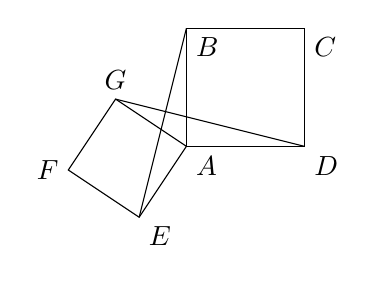
\begin{tikzpicture}[scale=0.3]
                \coordinate[label=below right:{$A$}] (A) at (0,0);
                \coordinate[label=below right:{$B$}] (B) at (0,5);
                \coordinate[label=below right:{$C$}] (C) at (5,5);
                \coordinate[label=below right:{$D$}] (D) at (5,0);
                \coordinate[label=below right:{$E$}] (E) at (-2,-3);
                \coordinate[label=left:{$F$}] (F) at (-5,-1);
                \coordinate[label=above:{$G$}] (G) at (-3,2);
                \draw (A) -- (B) -- (C) -- (D) -- cycle;
                \draw (A) -- (E) -- (F) -- (G) -- cycle;
                \draw (E) -- (B);
                \draw (G) -- (D);
            \end{tikzpicture}
        }\qquad\quad
        \subfigure[(第8题)]{
            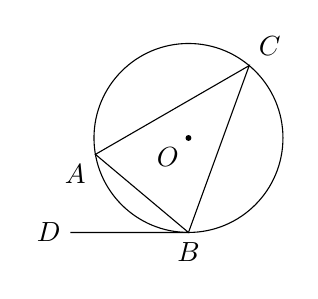
\begin{tikzpicture}[scale=0.3]
                \coordinate[label=below left:{$A$}] (A) at (-3.93923,3.30541);
                \coordinate[label=below:{$B$}] (B) at (0,0);
                \coordinate[label=above right:{$C$}] (C) at (2.57115,7.06418);
                \coordinate[label=left:{$D$}] (D) at (-5,0);
                \coordinate[label=below left:{$O$}] (O) at (0,4);
                \draw (O) circle (4);
                \filldraw (O) circle (0.1);
                \draw (D) -- (B) -- (A) -- (C) -- (B);
            \end{tikzpicture}
        }\qquad\qquad
        \subfigure[(第9题)]{
            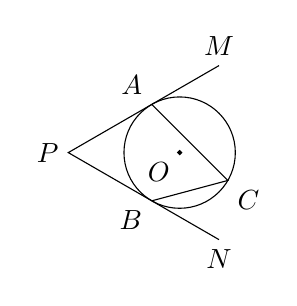
\begin{tikzpicture}[scale=0.5]
                \coordinate[label=below left:{$O$}] (O) at (0,0);
                \coordinate[label=above left:{$A$}] (A) at (-0.70711,1.22474);
                \coordinate[label=below left:{$B$}] (B) at (-0.70711,-1.22474);
                \coordinate[label=below right:{$C$}] (C) at (1.22474,-0.70711);
                \coordinate[label=left:{$P$}] (P) at (-2.82843,0);
                \coordinate[label=above:{$M$}] (M) at (1,2.21034);
                \coordinate[label=below:{$N$}] (N) at (1,-2.21034);
                \draw (O) circle (1.41421);
                \draw (M) -- (P) -- (N);
                \draw (A) -- (C) -- (B);
                \filldraw (O) circle (0.05);
            \end{tikzpicture}
        }
    \end{figure}
    \question 已知实数$t$满足当$-5 \leq x \leq 1$时,抛物线$y=tx^2-x$与折线$y=4t|x|-t+3$恰有$2$个公共点.若$t$是一个非零整数,则符合条件的$t$有(~~~~~~~)个.
    \onp{$0$}{$1$}{$2$}{$3$}
\end{questions}

\begin{questions}{\complitingintroduction}
    \question 已知点$(2,m)$和点$(n,-1)$关于原点中心对称,那么代数式$m+n$的值是\complitingline.
    \question 抛物线$y=-2x^2-6x+9$的顶点是\complitingline.
    \question 记点$O$和点$I$分别为$\Delta ABC$的外心和内心,若$\angle AOB=70^{\circ}$,则$\angle AIB=$\complitingline.
    \question “标记重捕法”是种群密度的常用调查方法之一,在一个鱼塘里随机抓取$24$条鱼标上记号后放回鱼塘,一段时间后重新抓$18$条鱼,发现其中有$4$条有记号,据此可估计该鱼塘内鱼的数量是\complitingline 条.
    \question 已知三个实数$a$、$b$、$c$之间满足
    $\begin{cases}
        |a| \geq |b| \\
        c > 0 \\
        4a+2b+c = 0
    \end{cases}$,则有下列说法:
    \begin{subsubquestions}
        \subsubquestion $a+b+c>0$;
        \subsubquestion $2a+c<0$;
        \subsubquestion 已知$A(x_1,y_1)$、$B(x_2,y_2)$是抛物线$y=ax^2+bx+c$上两点,且满足$x_1<x_2$.那么若$x_1+x_2>1$,则有$y_1>y_2$;
        \subsubquestion 当$c=2$时,对任意的$-2<q<0$,不等式$aq^2-(b+1)q+c-2 \geq 0$恒成立.
    \end{subsubquestions}
    其中正确的是\complitingline.
    \question 如图,正方形$ABCD$的边长为$4$,将线段$AD$绕点$D$顺时针旋转得到线段$PD$,使点$P$落在正方形$ABCD$内.过$P$作$PQ \bot AD$于$Q$,连$CD$的中点$T$和$\Delta PDQ$的内心$I$,则当$\angle ITD$最大时,$IT$的长度为\complitingline.
    \begin{figure}[!htb]
        \raggedleft
        \subfigure[(第16题)]{
            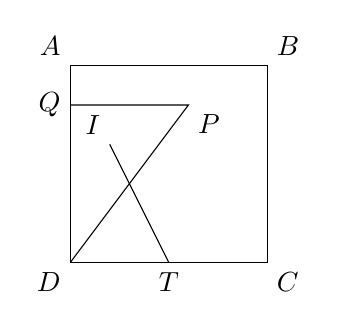
\begin{tikzpicture}[scale=0.5]
                \coordinate[label=above left:{$A$}] (A) at (0,5);
                \coordinate[label=above right:{$B$}] (B) at (5,5);
                \coordinate[label=below right:{$C$}] (C) at (5,0);
                \coordinate[label=below left:{$D$}] (D) at (0,0);
                \coordinate[label=below right:{$P$}] (P) at (3,4);
                \coordinate[label=left:{$Q$}] (Q) at (0,4);
                \coordinate[label=below:{$T$}] (T) at (2.5,0);
                \coordinate[label=above left:{$I$}] (I) at (1,3);
                \draw (A) -- (B) -- (C) -- (D) -- cycle;
                \draw (D) -- (P) -- (Q);
                \draw (T) -- (I);
            \end{tikzpicture}
        }
    \end{figure}
\end{questions}

\begin{questions}{\answeringintroduction}
    \question 已知关于$x$的一元二次方程$ax^2+bx+c=0$有一个根为$x=1$,且$a$、$b$满足$b=\sqrt{a-2}+\sqrt{2-a}-3$,解关于$y$的方程$\frac{1}{4}y^2-c=0$.
    \addemptyline\addemptyline
    \question 如图,在等边$\Delta ABC$中,$E$是$BC$上一点,连$AE$,将$\Delta ABE$绕点$A$旋转至$\Delta ACF$处,连$EF$.
    \begin{subquestions}
        \subquestion 判断$\Delta AEF$的形状并说明理由.
        \subquestion 若$BE=1$、$CE=2$,求$\Delta CEF$的面积.
    \end{subquestions}
    \begin{figure}[!htb]
        \raggedleft
        \subfigure[(第18题)]{
            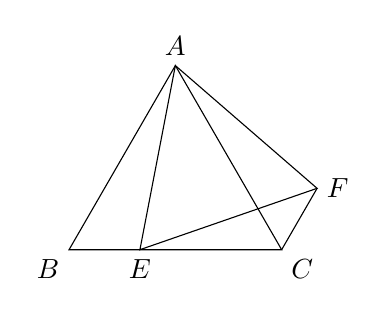
\begin{tikzpicture}[scale=0.45]
                \coordinate[label=above:{$A$}] (A) at (3,5.19615);
                \coordinate[label=below left:{$B$}] (B) at (0,0);
                \coordinate[label=below right:{$C$}] (C) at (6,0);
                \coordinate[label=below:{$E$}] (E) at (2,0);
                \coordinate[label=right:{$F$}] (F) at (7,1.73205);
                \draw (A) -- (B) -- (C) -- cycle;
                \draw (A) -- (E) -- (F) -- cycle;
                \draw (C) -- (F);
            \end{tikzpicture}
        }
    \end{figure}
    \question 一个不透明的袋子里装有四个球,四个球分别标有$2$、$3$、$4$、$6$四个数字,除标号不同外,四个球在各方面完全一样.现从袋中随机摸出$2$个球.
    \begin{subquestions}
        \subquestion 若每次摸出球后都放回袋中,直接写出两球的标号之积为奇数的概率是\complitingline.
        \subquestion 若每次摸出球后都不放回袋,求两球的标号互质(除$1$外没有公因数)的概率.
    \end{subquestions}
    \newpage
    \question 如图,边长为$2\sqrt{3}$的等边三角形$ABC$内接于$\odot O$,$D$是$\wideparen{AB}$上一点,连$CD$、$AD$、$BD$,有$\angle ACD=45^{\circ}$.
    \begin{subquestions}
        \subquestion 直接写出$\wideparen{{DB}^{l}}$的值和$\wideparen{AD}$与弦$AD$所围成区域的面积$S$.
        \subquestion 求$BD+DC$的值.
    \end{subquestions}
    \begin{figure}[!htb]
        \raggedleft
        \subfigure[(第20题)]{
            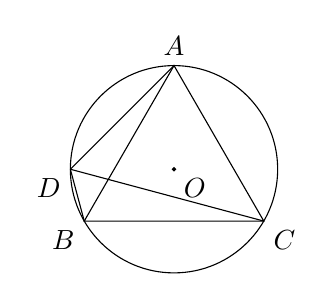
\begin{tikzpicture}[scale=0.38]
                \coordinate[label=above:{$A$}] (A) at (3,5.19615);
                \coordinate[label=below left:{$B$}] (B) at (0,0);
                \coordinate[label=below right:{$C$}] (C) at (6,0);
                \coordinate[label=below left:{$D$}] (D) at (-0.46410,1.73205);
                \coordinate[label=below right:{$O$}] (O) at (3,1.73205);
                \draw (A) -- (B) -- (C) -- cycle;
                \filldraw (O) circle (0.05);
                \draw (O) circle (3.46410);
                \draw (A) -- (D);
                \draw (B) -- (D);
                \draw (C) -- (D);
            \end{tikzpicture}
        }
    \end{figure}
    \question 如图是由小正方形组成的$7 \times 7$网格,每个小正方形的顶点叫做格点.已知$\odot O$交格点于$B$、$C$,交网格线于点$A$,连$AB$、$AC$.仅用无刻度的直尺在给定网格中完成画图,其中作图过程用虚线,作图结果用实线:
    \begin{subquestions}
        \subquestion 作弦$AD$平分$\angle BAC$.
        \subquestion 连$BD$,在弦$AD$上作点$E$,使得$ED=BD$.
        \subquestion 作弦$AF$与$BD$平行.
    \end{subquestions}
    \begin{figure}[!htb]
        \raggedleft
        \subfigure[(第21题)]{
            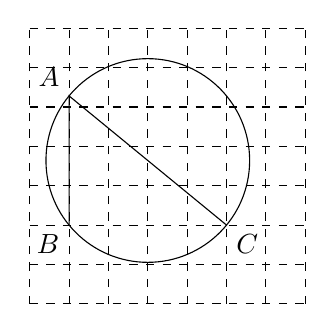
\begin{tikzpicture}[scale=0.5]
                \draw[step=1,dashed] (-1,-2) grid (6,5);
                \coordinate[label=below right:{$C$}] (C) at (4,0);
                \coordinate[label=above left:{$A$}] (A) at (0,3.28083);
                \coordinate[label=below left:{$B$}] (B) at (0,0);
                \draw (2,1.64042) circle (2.58669);
                \draw (B) -- (A) -- (C);
            \end{tikzpicture}}
    \end{figure}
    \question 如图是某兴趣小组设计的游戏装置.在一个水平滑道上,小球甲在被加速后以$40$cm/s的初速度从滑道$A$点出发,沿滑道向右作匀减速直线运动,其滑行距离$s$(cm)、瞬时速度$v_1$(cm/s)与滑行时间$t_1$(s)之间的关系如下表所示:
    \begin{table}[!htbp]
        \centering
        \begin{tabularx}{0.5\textwidth}[!htb]{|m{3.8cm}<{\centering}|*{4}{>{\centering\arraybackslash}X|}} \hline
            滑行时间$t_1$(s)& $0$ & $0.5$ & $1$ & $\cdots$ \\ \hline
            滑行距离$s$(cm)& $0$ & $17.5$ & $30$ & $\cdots$ \\ \hline
            瞬时速度$v_1$(cm/s) & $40$ & $30$ & $20$ & $\cdots$ \\ \hline
        \end{tabularx}
    \end{table}\par
    \qquad 与此同时,在滑道$B$点处有另一个静止的小球乙被一根绳子悬挂着,绳长$OB=4$cm,且小球乙正好与滑道相切.当小球甲撞到小球乙时,其速度$v_1$将全部传给小球乙,成为乙的初速度$v_2$.随后,小球乙将绕点$O$、以$OB$为半径作圆周运动,其上升高度$h$(cm)和运动时间$t_2$(s)之间满足$h=v_2t_2-2{t_2}^2$.小球乙在上升到最高点$D$后摆回至点$B$,随后停止运动.\par
    \qquad 现已知$s$与$t_1$、$v_1$与$t_1$之间的函数关系是我们学过的函数,若不计两小球的大小,回答下列问题:
    \begin{subquestions}
        \subquestion 直接写出$s$与$t_1$、$v_1$与$t_1$之间的函数关系式(不必写出自变量的取值范围).
        \subquestion 若小球乙共运动了$3$秒,求$AB$的长度.
        \subquestion 若$\angle DOB=60^{\circ}$,求$AB$的长度.
    \end{subquestions}
    \begin{figure}[!htbp]
        \centering
        \begin{tikzpicture}[scale=0.5,>=Stealth]
            \draw (-7,0) -- (10,0);
            \draw (3,5) -- (9,5);
            \coordinate (B) at (4,1);
            \coordinate (D) at (7.46410,3);
            \node[above right] at (8.14711,3) {$D$};
            \node[above right] at (4.25,0.75) {$B$};
            \coordinate[label=above:{$O$}] (O) at (4,5);
            \draw (B) -- (O);
            \draw[densely dashed] (O) -- (D);
            \draw (4,0.5) circle (0.5);
            \draw (-5,0.5) circle (0.5);
            \node[above right] at (-4.75,0.75) {$A$};
            \draw[densely dashed] (7.89711,2.75) circle (0.5);
            \draw[densely dashed] (0,0.5) circle (0.5);
            \draw[->] (-3.6,1.1) -- (-2.6,1.1) node[above left] {$v_1$};
            \draw[densely dashed] (2.3,2.75) -- (7.5,2.75);
            \node[left] at (2.5,1.375) {$h$};
            \draw[<->] (2.5,0.1) -- (2.5,2.74);
            \draw[densely dashed] (4,0.5) arc (270:330:4.5);
        \end{tikzpicture}
        \caption*{(第22题)}
    \end{figure}
    \question 如图,菱形$ABCD$的边长为$2\sqrt{5}$,且$\angle ABC=60^{\circ}$,等边$\Delta AEF$绕点$A$在菱形$ABCD$内部旋转,连$BE$和$DF$.
    \begin{subquestions}
        \subquestion 如图1,当$B$、$E$、$F$三点共线时,求证:$\angle ABE=\angle DAF$.
        \subquestion 如图2,当$\angle ABE+\angle ADF=75^{\circ}$时,若$DF=2\sqrt{2}$,求线段$BE$的长.
        \subquestion 如图3,以$BA$、$BE$为边,作平行四边形$ABEP$,连$P$和$CD$中点$Q$,若等边$\Delta AEF$的边长为$3$,直接写出线段$PQ$长度的最小值.
    \end{subquestions}
    \begin{figure}[!htb]
        \centering
        \subfigure[(1)]{
            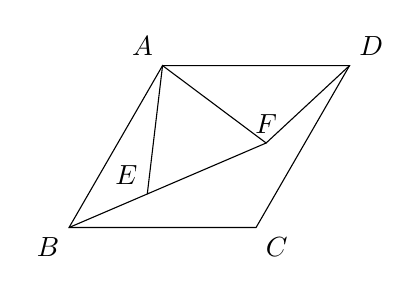
\begin{tikzpicture}[scale=0.475]
                \coordinate[label=above left:{$A$}] (A) at (2.5,4.33013);
                \coordinate[label=below left:{$B$}] (B) at (0,0);
                \coordinate[label=below right:{$C$}] (C) at (5,0);
                \coordinate[label=above right:{$D$}] (D) at (7.5,4.33013);
                \draw (A) -- (B) -- (C) -- (D) -- cycle;
                \coordinate[label=above left:{$E$}] (E) at (2.09151,0.89705);
                \coordinate[label=above:{$F$}] (F) at (5.26889,2.25983);
                \draw (A) -- (E) -- (F) -- cycle;
                \draw (B) -- (E);
                \draw (D) -- (F);
            \end{tikzpicture}
        } \qquad \qquad
        \subfigure[(2)]{
            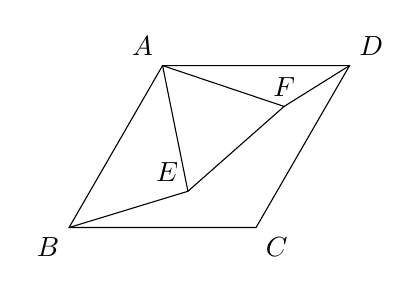
\begin{tikzpicture}[scale=0.475]
                \coordinate[label=above left:{$A$}] (A) at (2.5,4.33013);
                \coordinate[label=below left:{$B$}] (B) at (0,0);
                \coordinate[label=below right:{$C$}] (C) at (5,0);
                \coordinate[label=above right:{$D$}] (D) at (7.5,4.33013);
                \draw (A) -- (B) -- (C) -- (D) -- cycle;
                \coordinate[label=above left:{$E$}] (E) at (3.17839,0.96984);
                \coordinate[label=above:{$F$}] (F) at (5.74929,3.23749);
                \draw (A) -- (E) -- (F) -- cycle;
                \draw (B) -- (E);
                \draw (D) -- (F);
            \end{tikzpicture}
        } \qquad \qquad
        \subfigure[(3)]{
            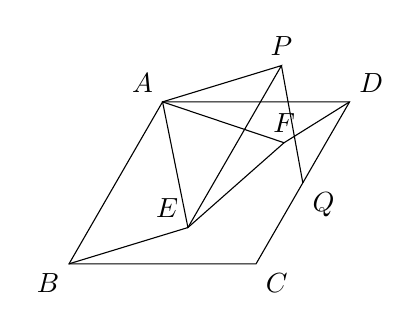
\begin{tikzpicture}[scale=0.475]
                \coordinate[label=above left:{$A$}] (A) at (2.5,4.33013);
                \coordinate[label=below left:{$B$}] (B) at (0,0);
                \coordinate[label=below right:{$C$}] (C) at (5,0);
                \coordinate[label=above right:{$D$}] (D) at (7.5,4.33013);
                \draw (A) -- (B) -- (C) -- (D) -- cycle;
                \coordinate[label=above left:{$E$}] (E) at (3.17839,0.96984);
                \coordinate[label=above:{$F$}] (F) at (5.74929,3.23749);
                \draw (A) -- (E) -- (F) -- cycle;
                \draw (B) -- (E);
                \draw (D) -- (F);
                \coordinate[label=above:{$P$}] (P) at (5.67839,5.29997);
                \coordinate[label=below right:{$Q$}] (Q) at (6.25,2.16506);
                \draw (A) -- (P) -- (E);
                \draw (P) -- (Q);
            \end{tikzpicture}
        }
        \caption*{(第23题)}
    \end{figure}
    \question 定义:与一条抛物线有且仅有一个交点,且不与这条抛物线的对称轴平行的直线为这条抛物线的\textbf{切线}. \\
    在平面直角坐标系$xOy$中,恒过点$F(0,2)$的动圆$\odot P$保持与$x$轴相切.记点$P$的运动轨迹为$\Gamma$.
    \begin{subquestions}
        \subquestion 已知$\Gamma$是一条常见的曲线.
        \begin{subsubquestions}
            \subsubquestion 当点$P$运动到$y$轴上时,点$P$的坐标是\complitingline;当$\odot P$与$y$轴相切时,点$P$的坐标是\complitingline.
            \subsubquestion 根据\circnum{1}的结果,直接写出$\Gamma$的解析式是\complitingline.
        \end{subsubquestions}
        \subquestion 如图1,作射线$OP$,求$\angle FOP$的最大值.
        \subquestion 如图2,作直线$PF$交$\Gamma$于点$Q$,分别过点$P$、$Q$作$\Gamma$的切线,记这两条切线的交点为$T$,连$TF$,求证:$TF \bot PQ$.
    \end{subquestions}
    \begin{figure}[!htb]
        \centering
        \subfigure[(1)]{
            \begin{tikzpicture}[>=Stealth,scale=0.65]
                \draw[->] (-4,0) -- (4,0) node[below] {$x$};
                \draw[->] (0,-1) -- (0,5) node[right] {$y$};
                \coordinate[label=below right:{$O$}] (O) at (0,0);
                \coordinate[label=right:{$F$}] (F) at (0,2);
                \draw (-4,5) parabola bend (0,1) (4,5);
                \coordinate[label=right:{$P$}] (P) at (-3,3.25);
                \draw (P) circle (3.25);
                \draw (O) -- (-4,4.3333);
            \end{tikzpicture}
        }\qquad\qquad
        \subfigure[(2)]{
            \begin{tikzpicture}[>=Stealth,scale=0.65]
                \draw[->] (-4,0) -- (4,0) node[below] {$x$};
                \draw[->] (0,-1) -- (0,5) node[right] {$y$};
                \coordinate[label=below right:{$O$}] (O) at (0,0);
                \coordinate[label=right:{$F$}] (F) at (0,2);
                \draw (-4,5) parabola bend (0,1) (4,5);
                \coordinate[label=below left:{$P$}] (P) at (-3,3.25);
                \coordinate[label=below right:{$Q$}] (Q) at (1.333333,1.444444);
                \coordinate[label=below:{$T$}] (T) at (-0.83333,0);
                \draw (P) -- (Q) -- (T) -- cycle;
                \draw (F) -- (T);
            \end{tikzpicture}
        }
        \caption*{(第24题)}
    \end{figure}
\end{questions}
\end{document}